\setlength{\intextsep}{-.9pt}
\begin{figure}
  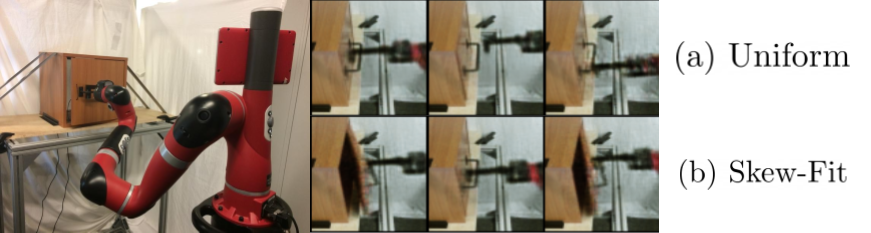
\includegraphics[width=\linewidth]{skewfit/figures/realworldwithsamples.png}
  \fcaption{
  Left: Robot learning to open a door with \METHOD, without any task reward.
  Right: Samples from a goal distribution when using (a) uniform and (b) \METHOD sampling.
  When used as goals, the diverse samples from \METHOD encourage the robot to practice opening the door more frequently.
  }
  \label{fig:offline-sk-real}
\end{figure}
Reinforcement learning (RL) provides an appealing formalism for automated learning of behavioral skills, but separately learning every potentially useful skill becomes prohibitively time consuming, both in terms of the experience required for the agent and the effort required for the user to design reward functions for each behavior.
What if we could instead design an unsupervised RL algorithm that automatically explores the environment and iteratively distills this experience into general-purpose policies that can accomplish new user-specified tasks at test time?

In the absence of any prior knowledge, an effective exploration scheme is one that visits as many states as possible, allowing a policy to autonomously prepare for user-specified tasks that it might see at test time.
We can formalize the problem of visiting as many states as possible as one of maximizing the \emph{state entropy} $\gH(\SF)$ under the current policy.\stepcounter{footnote}\footnote{We consider the distribution over terminal states in a finite horizon task  and believe this work can be extended to infinite horizon stationary distributions.}
Unfortunately, optimizing this objective alone does not result in a policy that can solve new tasks: it only knows how to maximize state entropy.
In other words, to develop principled unsupervised RL algorithms that result in useful policies, maximizing $\gH(\SF)$ is not enough.
We need a mechanism that allows us to reuse the resulting policy to achieve new tasks at test-time.

We argue that this can be accomplished by performing \textit{goal-directed exploration}:
a policy should autonomously visit as many states as possible, but after autonomous exploration, a user should be able to reuse this policy by giving it a goal $\G$ that corresponds to a state that it must reach.
While not all test-time tasks can be expressed as reaching a goal state, a wide range of tasks can be represented in this way.
Mathematically, the goal-conditioned policy should minimize the conditional entropy over the states given a goal, $\gH(\SF \mid \G)$, so that there is little uncertainty over its state given a commanded goal.
This objective provides us with a principled way to train a policy to explore all states (maximize $\gH(\SF)$) such that the state that is reached can be determined by commanding goals (minimize $\gH(\SF \mid \G)$).

Directly optimizing this objective is in general intractable, since it requires optimizing the entropy of the marginal state distribution, $\gH(\SF)$.
However, we can sidestep this issue by noting that the objective is the mutual information between the state and the goal, $I(\SF; \G)$, which can be written as:
{
  \setlength{\abovedisplayskip}{18pt}%
  \setlength{\belowdisplayskip}{0pt}%
  \setlength{\abovedisplayshortskip}{18pt}%
  \setlength{\belowdisplayshortskip}{0pt}
\begin{align}
    \label{eq:hg-hgs}
    \gH(\SF) - \gH(\SF|\G)
    =
    I(\SF; \G)
    =
    \gH(\G) - \gH(\G|\SF).
\end{align}
}

\Eqref{eq:hg-hgs} thus gives an equivalent objective for an unsupervised RL algorithm:
the agent should set diverse goals, maximizing $\gH(\G)$, and learn how to reach them, minimizing $\gH(\G \mid \SF)$.

While learning to reach goals is the typical objective studied in goal-conditioned RL~\citep{kaelbling1993goals,andrychowicz2017her}, setting goals that have maximum diversity is crucial for effectively learning to reach all possible states.
Acquiring such a maximum-entropy goal distribution is challenging in environments with complex, high-dimensional state spaces, where even knowing which states are valid presents a major challenge.
For example, in image-based domains, a uniform goal distribution requires sampling uniformly from the set of realistic images, which in general is unknown a priori.

Our paper makes the following contributions.
First, we propose a principled objective for unsupervised RL, based on \autoref{eq:hg-hgs}.
While a number of prior works ignore the $\gH(\G)$ term, we argue that jointly optimizing the entire quantity is needed to develop effective exploration.
Second, we present a general algorithm called \METHOD and prove that under regularity conditions \METHOD learns a sequence of generative models that converges to a uniform distribution over the goal space, even when the set of valid states is unknown (e.g., as in the case of images).
Third, we describe a concrete implementation of \METHOD and empirically demonstrate that this method achieves state of the art results compared to a large number of prior methods for goal reaching with visually indicated goals, including a real-world manipulation task, which requires a robot to learn to open a door from scratch in about five hours, directly from images, and without any manually-designed reward function.